% Created by tikzDevice version 0.12 on 2019-04-15 16:15:58
% !TEX encoding = UTF-8 Unicode
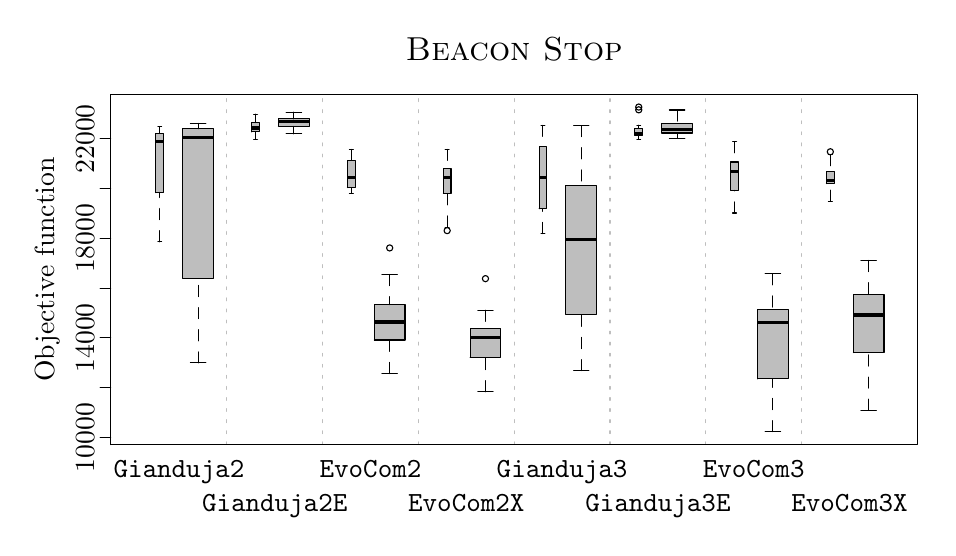
\begin{tikzpicture}[x=1pt,y=1pt]
\definecolor{fillColor}{RGB}{255,255,255}
\path[use as bounding box,fill=fillColor,fill opacity=0.00] (0,0) rectangle (325.21,180.67);
\begin{scope}
\path[clip] ( 30.00, 30.00) rectangle (321.61,156.67);
\definecolor{fillColor}{RGB}{190,190,190}

\path[fill=fillColor] ( 46.34,121.11) --
	( 49.11,121.11) --
	( 49.11,142.47) --
	( 46.34,142.47) --
	cycle;
\definecolor{drawColor}{RGB}{0,0,0}

\path[draw=drawColor,line width= 1.2pt,line join=round] ( 46.34,139.60) -- ( 49.11,139.60);

\path[draw=drawColor,line width= 0.4pt,dash pattern=on 4pt off 4pt ,line join=round,line cap=round] ( 47.72,103.31) -- ( 47.72,121.11);

\path[draw=drawColor,line width= 0.4pt,dash pattern=on 4pt off 4pt ,line join=round,line cap=round] ( 47.72,144.87) -- ( 47.72,142.47);

\path[draw=drawColor,line width= 0.4pt,line join=round,line cap=round] ( 47.03,103.31) -- ( 48.42,103.31);

\path[draw=drawColor,line width= 0.4pt,line join=round,line cap=round] ( 47.03,144.87) -- ( 48.42,144.87);

\path[draw=drawColor,line width= 0.4pt,line join=round,line cap=round] ( 46.34,121.11) --
	( 49.11,121.11) --
	( 49.11,142.47) --
	( 46.34,142.47) --
	( 46.34,121.11);

\path[fill=fillColor] ( 56.03, 90.09) --
	( 67.11, 90.09) --
	( 67.11,144.16) --
	( 56.03,144.16) --
	cycle;

\path[draw=drawColor,line width= 1.2pt,line join=round] ( 56.03,141.07) -- ( 67.11,141.07);

\path[draw=drawColor,line width= 0.4pt,dash pattern=on 4pt off 4pt ,line join=round,line cap=round] ( 61.57, 59.53) -- ( 61.57, 90.09);

\path[draw=drawColor,line width= 0.4pt,dash pattern=on 4pt off 4pt ,line join=round,line cap=round] ( 61.57,146.04) -- ( 61.57,144.16);

\path[draw=drawColor,line width= 0.4pt,line join=round,line cap=round] ( 58.80, 59.53) -- ( 64.34, 59.53);

\path[draw=drawColor,line width= 0.4pt,line join=round,line cap=round] ( 58.80,146.04) -- ( 64.34,146.04);

\path[draw=drawColor,line width= 0.4pt,line join=round,line cap=round] ( 56.03, 90.09) --
	( 67.11, 90.09) --
	( 67.11,144.16) --
	( 56.03,144.16) --
	( 56.03, 90.09);

\path[fill=fillColor] ( 80.96,143.06) --
	( 83.73,143.06) --
	( 83.73,146.42) --
	( 80.96,146.42) --
	cycle;

\path[draw=drawColor,line width= 1.2pt,line join=round] ( 80.96,144.44) -- ( 83.73,144.44);

\path[draw=drawColor,line width= 0.4pt,dash pattern=on 4pt off 4pt ,line join=round,line cap=round] ( 82.34,140.36) -- ( 82.34,143.06);

\path[draw=drawColor,line width= 0.4pt,dash pattern=on 4pt off 4pt ,line join=round,line cap=round] ( 82.34,149.38) -- ( 82.34,146.42);

\path[draw=drawColor,line width= 0.4pt,line join=round,line cap=round] ( 81.65,140.36) -- ( 83.03,140.36);

\path[draw=drawColor,line width= 0.4pt,line join=round,line cap=round] ( 81.65,149.38) -- ( 83.03,149.38);

\path[draw=drawColor,line width= 0.4pt,line join=round,line cap=round] ( 80.96,143.06) --
	( 83.73,143.06) --
	( 83.73,146.42) --
	( 80.96,146.42) --
	( 80.96,143.06);

\path[fill=fillColor] ( 90.65,145.00) --
	(101.73,145.00) --
	(101.73,147.76) --
	( 90.65,147.76) --
	cycle;

\path[draw=drawColor,line width= 1.2pt,line join=round] ( 90.65,146.79) -- (101.73,146.79);

\path[draw=drawColor,line width= 0.4pt,dash pattern=on 4pt off 4pt ,line join=round,line cap=round] ( 96.19,142.34) -- ( 96.19,145.00);

\path[draw=drawColor,line width= 0.4pt,dash pattern=on 4pt off 4pt ,line join=round,line cap=round] ( 96.19,150.16) -- ( 96.19,147.76);

\path[draw=drawColor,line width= 0.4pt,line join=round,line cap=round] ( 93.42,142.34) -- ( 98.96,142.34);

\path[draw=drawColor,line width= 0.4pt,line join=round,line cap=round] ( 93.42,150.16) -- ( 98.96,150.16);

\path[draw=drawColor,line width= 0.4pt,line join=round,line cap=round] ( 90.65,145.00) --
	(101.73,145.00) --
	(101.73,147.76) --
	( 90.65,147.76) --
	( 90.65,145.00);

\path[fill=fillColor] (115.57,122.87) --
	(118.34,122.87) --
	(118.34,132.71) --
	(115.57,132.71) --
	cycle;

\path[draw=drawColor,line width= 1.2pt,line join=round] (115.57,126.45) -- (118.34,126.45);

\path[draw=drawColor,line width= 0.4pt,dash pattern=on 4pt off 4pt ,line join=round,line cap=round] (116.96,120.82) -- (116.96,122.87);

\path[draw=drawColor,line width= 0.4pt,dash pattern=on 4pt off 4pt ,line join=round,line cap=round] (116.96,136.64) -- (116.96,132.71);

\path[draw=drawColor,line width= 0.4pt,line join=round,line cap=round] (116.27,120.82) -- (117.65,120.82);

\path[draw=drawColor,line width= 0.4pt,line join=round,line cap=round] (116.27,136.64) -- (117.65,136.64);

\path[draw=drawColor,line width= 0.4pt,line join=round,line cap=round] (115.57,122.87) --
	(118.34,122.87) --
	(118.34,132.71) --
	(115.57,132.71) --
	(115.57,122.87);

\path[fill=fillColor] (125.27, 67.80) --
	(136.34, 67.80) --
	(136.34, 80.60) --
	(125.27, 80.60) --
	cycle;

\path[draw=drawColor,line width= 1.2pt,line join=round] (125.27, 74.27) -- (136.34, 74.27);

\path[draw=drawColor,line width= 0.4pt,dash pattern=on 4pt off 4pt ,line join=round,line cap=round] (130.81, 55.69) -- (130.81, 67.80);

\path[draw=drawColor,line width= 0.4pt,dash pattern=on 4pt off 4pt ,line join=round,line cap=round] (130.81, 91.46) -- (130.81, 80.60);

\path[draw=drawColor,line width= 0.4pt,line join=round,line cap=round] (128.04, 55.69) -- (133.57, 55.69);

\path[draw=drawColor,line width= 0.4pt,line join=round,line cap=round] (128.04, 91.46) -- (133.57, 91.46);

\path[draw=drawColor,line width= 0.4pt,line join=round,line cap=round] (125.27, 67.80) --
	(136.34, 67.80) --
	(136.34, 80.60) --
	(125.27, 80.60) --
	(125.27, 67.80);

\path[draw=drawColor,line width= 0.4pt,line join=round,line cap=round] (130.81,101.08) circle (  1.12);

\path[fill=fillColor] (150.19,120.82) --
	(152.96,120.82) --
	(152.96,129.79) --
	(150.19,129.79) --
	cycle;

\path[draw=drawColor,line width= 1.2pt,line join=round] (150.19,126.49) -- (152.96,126.49);

\path[draw=drawColor,line width= 0.4pt,dash pattern=on 4pt off 4pt ,line join=round,line cap=round] (151.58,108.62) -- (151.58,120.82);

\path[draw=drawColor,line width= 0.4pt,dash pattern=on 4pt off 4pt ,line join=round,line cap=round] (151.58,136.70) -- (151.58,129.79);

\path[draw=drawColor,line width= 0.4pt,line join=round,line cap=round] (150.88,108.62) -- (152.27,108.62);

\path[draw=drawColor,line width= 0.4pt,line join=round,line cap=round] (150.88,136.70) -- (152.27,136.70);

\path[draw=drawColor,line width= 0.4pt,line join=round,line cap=round] (150.19,120.82) --
	(152.96,120.82) --
	(152.96,129.79) --
	(150.19,129.79) --
	(150.19,120.82);

\path[draw=drawColor,line width= 0.4pt,line join=round,line cap=round] (151.58,107.33) circle (  1.12);

\path[fill=fillColor] (159.88, 61.61) --
	(170.96, 61.61) --
	(170.96, 72.10) --
	(159.88, 72.10) --
	cycle;

\path[draw=drawColor,line width= 1.2pt,line join=round] (159.88, 68.67) -- (170.96, 68.67);

\path[draw=drawColor,line width= 0.4pt,dash pattern=on 4pt off 4pt ,line join=round,line cap=round] (165.42, 49.12) -- (165.42, 61.61);

\path[draw=drawColor,line width= 0.4pt,dash pattern=on 4pt off 4pt ,line join=round,line cap=round] (165.42, 78.55) -- (165.42, 72.10);

\path[draw=drawColor,line width= 0.4pt,line join=round,line cap=round] (162.65, 49.12) -- (168.19, 49.12);

\path[draw=drawColor,line width= 0.4pt,line join=round,line cap=round] (162.65, 78.55) -- (168.19, 78.55);

\path[draw=drawColor,line width= 0.4pt,line join=round,line cap=round] (159.88, 61.61) --
	(170.96, 61.61) --
	(170.96, 72.10) --
	(159.88, 72.10) --
	(159.88, 61.61);

\path[draw=drawColor,line width= 0.4pt,line join=round,line cap=round] (165.42, 89.98) circle (  1.12);

\path[fill=fillColor] (184.81,115.25) --
	(187.58,115.25) --
	(187.58,137.57) --
	(184.81,137.57) --
	cycle;

\path[draw=drawColor,line width= 1.2pt,line join=round] (184.81,126.65) -- (187.58,126.65);

\path[draw=drawColor,line width= 0.4pt,dash pattern=on 4pt off 4pt ,line join=round,line cap=round] (186.19,106.29) -- (186.19,115.25);

\path[draw=drawColor,line width= 0.4pt,dash pattern=on 4pt off 4pt ,line join=round,line cap=round] (186.19,145.38) -- (186.19,137.57);

\path[draw=drawColor,line width= 0.4pt,line join=round,line cap=round] (185.50,106.29) -- (186.88,106.29);

\path[draw=drawColor,line width= 0.4pt,line join=round,line cap=round] (185.50,145.38) -- (186.88,145.38);

\path[draw=drawColor,line width= 0.4pt,line join=round,line cap=round] (184.81,115.25) --
	(187.58,115.25) --
	(187.58,137.57) --
	(184.81,137.57) --
	(184.81,115.25);

\path[fill=fillColor] (194.50, 77.08) --
	(205.58, 77.08) --
	(205.58,123.51) --
	(194.50,123.51) --
	cycle;

\path[draw=drawColor,line width= 1.2pt,line join=round] (194.50,104.24) -- (205.58,104.24);

\path[draw=drawColor,line width= 0.4pt,dash pattern=on 4pt off 4pt ,line join=round,line cap=round] (200.04, 56.74) -- (200.04, 77.08);

\path[draw=drawColor,line width= 0.4pt,dash pattern=on 4pt off 4pt ,line join=round,line cap=round] (200.04,145.28) -- (200.04,123.51);

\path[draw=drawColor,line width= 0.4pt,line join=round,line cap=round] (197.27, 56.74) -- (202.81, 56.74);

\path[draw=drawColor,line width= 0.4pt,line join=round,line cap=round] (197.27,145.28) -- (202.81,145.28);

\path[draw=drawColor,line width= 0.4pt,line join=round,line cap=round] (194.50, 77.08) --
	(205.58, 77.08) --
	(205.58,123.51) --
	(194.50,123.51) --
	(194.50, 77.08);

\path[fill=fillColor] (219.43,141.74) --
	(222.19,141.74) --
	(222.19,144.31) --
	(219.43,144.31) --
	cycle;

\path[draw=drawColor,line width= 1.2pt,line join=round] (219.43,142.40) -- (222.19,142.40);

\path[draw=drawColor,line width= 0.4pt,dash pattern=on 4pt off 4pt ,line join=round,line cap=round] (220.81,140.36) -- (220.81,141.74);

\path[draw=drawColor,line width= 0.4pt,dash pattern=on 4pt off 4pt ,line join=round,line cap=round] (220.81,145.40) -- (220.81,144.31);

\path[draw=drawColor,line width= 0.4pt,line join=round,line cap=round] (220.12,140.36) -- (221.50,140.36);

\path[draw=drawColor,line width= 0.4pt,line join=round,line cap=round] (220.12,145.40) -- (221.50,145.40);

\path[draw=drawColor,line width= 0.4pt,line join=round,line cap=round] (219.43,141.74) --
	(222.19,141.74) --
	(222.19,144.31) --
	(219.43,144.31) --
	(219.43,141.74);

\path[draw=drawColor,line width= 0.4pt,line join=round,line cap=round] (220.81,150.98) circle (  1.12);

\path[draw=drawColor,line width= 0.4pt,line join=round,line cap=round] (220.81,151.98) circle (  1.12);

\path[fill=fillColor] (229.12,142.59) --
	(240.20,142.59) --
	(240.20,145.92) --
	(229.12,145.92) --
	cycle;

\path[draw=drawColor,line width= 1.2pt,line join=round] (229.12,143.93) -- (240.20,143.93);

\path[draw=drawColor,line width= 0.4pt,dash pattern=on 4pt off 4pt ,line join=round,line cap=round] (234.66,140.78) -- (234.66,142.59);

\path[draw=drawColor,line width= 0.4pt,dash pattern=on 4pt off 4pt ,line join=round,line cap=round] (234.66,150.90) -- (234.66,145.92);

\path[draw=drawColor,line width= 0.4pt,line join=round,line cap=round] (231.89,140.78) -- (237.43,140.78);

\path[draw=drawColor,line width= 0.4pt,line join=round,line cap=round] (231.89,150.90) -- (237.43,150.90);

\path[draw=drawColor,line width= 0.4pt,line join=round,line cap=round] (229.12,142.59) --
	(240.20,142.59) --
	(240.20,145.92) --
	(229.12,145.92) --
	(229.12,142.59);

\path[fill=fillColor] (254.04,121.86) --
	(256.81,121.86) --
	(256.81,132.11) --
	(254.04,132.11) --
	cycle;

\path[draw=drawColor,line width= 1.2pt,line join=round] (254.04,128.66) -- (256.81,128.66);

\path[draw=drawColor,line width= 0.4pt,dash pattern=on 4pt off 4pt ,line join=round,line cap=round] (255.43,113.71) -- (255.43,121.86);

\path[draw=drawColor,line width= 0.4pt,dash pattern=on 4pt off 4pt ,line join=round,line cap=round] (255.43,139.48) -- (255.43,132.11);

\path[draw=drawColor,line width= 0.4pt,line join=round,line cap=round] (254.73,113.71) -- (256.12,113.71);

\path[draw=drawColor,line width= 0.4pt,line join=round,line cap=round] (254.73,139.48) -- (256.12,139.48);

\path[draw=drawColor,line width= 0.4pt,line join=round,line cap=round] (254.04,121.86) --
	(256.81,121.86) --
	(256.81,132.11) --
	(254.04,132.11) --
	(254.04,121.86);

\path[fill=fillColor] (263.74, 53.78) --
	(274.81, 53.78) --
	(274.81, 78.81) --
	(263.74, 78.81) --
	cycle;

\path[draw=drawColor,line width= 1.2pt,line join=round] (263.74, 74.17) -- (274.81, 74.17);

\path[draw=drawColor,line width= 0.4pt,dash pattern=on 4pt off 4pt ,line join=round,line cap=round] (269.27, 34.69) -- (269.27, 53.78);

\path[draw=drawColor,line width= 0.4pt,dash pattern=on 4pt off 4pt ,line join=round,line cap=round] (269.27, 91.73) -- (269.27, 78.81);

\path[draw=drawColor,line width= 0.4pt,line join=round,line cap=round] (266.50, 34.69) -- (272.04, 34.69);

\path[draw=drawColor,line width= 0.4pt,line join=round,line cap=round] (266.50, 91.73) -- (272.04, 91.73);

\path[draw=drawColor,line width= 0.4pt,line join=round,line cap=round] (263.74, 53.78) --
	(274.81, 53.78) --
	(274.81, 78.81) --
	(263.74, 78.81) --
	(263.74, 53.78);

\path[fill=fillColor] (288.66,124.29) --
	(291.43,124.29) --
	(291.43,128.74) --
	(288.66,128.74) --
	cycle;

\path[draw=drawColor,line width= 1.2pt,line join=round] (288.66,125.47) -- (291.43,125.47);

\path[draw=drawColor,line width= 0.4pt,dash pattern=on 4pt off 4pt ,line join=round,line cap=round] (290.04,117.96) -- (290.04,124.29);

\path[draw=drawColor,line width= 0.4pt,dash pattern=on 4pt off 4pt ,line join=round,line cap=round] (290.04,134.79) -- (290.04,128.74);

\path[draw=drawColor,line width= 0.4pt,line join=round,line cap=round] (289.35,117.96) -- (290.74,117.96);

\path[draw=drawColor,line width= 0.4pt,line join=round,line cap=round] (289.35,134.79) -- (290.74,134.79);

\path[draw=drawColor,line width= 0.4pt,line join=round,line cap=round] (288.66,124.29) --
	(291.43,124.29) --
	(291.43,128.74) --
	(288.66,128.74) --
	(288.66,124.29);

\path[draw=drawColor,line width= 0.4pt,line join=round,line cap=round] (290.04,135.83) circle (  1.12);

\path[fill=fillColor] (298.35, 63.28) --
	(309.43, 63.28) --
	(309.43, 84.31) --
	(298.35, 84.31) --
	cycle;

\path[draw=drawColor,line width= 1.2pt,line join=round] (298.35, 76.83) -- (309.43, 76.83);

\path[draw=drawColor,line width= 0.4pt,dash pattern=on 4pt off 4pt ,line join=round,line cap=round] (303.89, 42.41) -- (303.89, 63.28);

\path[draw=drawColor,line width= 0.4pt,dash pattern=on 4pt off 4pt ,line join=round,line cap=round] (303.89, 96.53) -- (303.89, 84.31);

\path[draw=drawColor,line width= 0.4pt,line join=round,line cap=round] (301.12, 42.41) -- (306.66, 42.41);

\path[draw=drawColor,line width= 0.4pt,line join=round,line cap=round] (301.12, 96.53) -- (306.66, 96.53);

\path[draw=drawColor,line width= 0.4pt,line join=round,line cap=round] (298.35, 63.28) --
	(309.43, 63.28) --
	(309.43, 84.31) --
	(298.35, 84.31) --
	(298.35, 63.28);
\definecolor{drawColor}{RGB}{190,190,190}

\path[draw=drawColor,line width= 0.4pt,dash pattern=on 1pt off 3pt ,line join=round,line cap=round] ( 71.96, 30.00) -- ( 71.96,156.67);

\path[draw=drawColor,line width= 0.4pt,dash pattern=on 1pt off 3pt ,line join=round,line cap=round] (106.57, 30.00) -- (106.57,156.67);

\path[draw=drawColor,line width= 0.4pt,dash pattern=on 1pt off 3pt ,line join=round,line cap=round] (141.19, 30.00) -- (141.19,156.67);

\path[draw=drawColor,line width= 0.4pt,dash pattern=on 1pt off 3pt ,line join=round,line cap=round] (175.81, 30.00) -- (175.81,156.67);

\path[draw=drawColor,line width= 0.4pt,dash pattern=on 1pt off 3pt ,line join=round,line cap=round] (210.42, 30.00) -- (210.42,156.67);

\path[draw=drawColor,line width= 0.4pt,dash pattern=on 1pt off 3pt ,line join=round,line cap=round] (245.04, 30.00) -- (245.04,156.67);

\path[draw=drawColor,line width= 0.4pt,dash pattern=on 1pt off 3pt ,line join=round,line cap=round] (279.66, 30.00) -- (279.66,156.67);
\end{scope}
\begin{scope}
\path[clip] (  0.00,  0.00) rectangle (325.21,180.67);
\definecolor{drawColor}{RGB}{0,0,0}

\node[text=drawColor,anchor=base,inner sep=0pt, outer sep=0pt, scale=  1.00] at ( 54.65, 18.00) {\texttt{Gianduja2}};

\node[text=drawColor,anchor=base,inner sep=0pt, outer sep=0pt, scale=  1.00] at (123.88, 18.00) {\texttt{EvoCom2}};

\node[text=drawColor,anchor=base,inner sep=0pt, outer sep=0pt, scale=  1.00] at (193.12, 18.00) {\texttt{Gianduja3}};

\node[text=drawColor,anchor=base,inner sep=0pt, outer sep=0pt, scale=  1.00] at (262.35, 18.00) {\texttt{EvoCom3}};

\node[text=drawColor,anchor=base,inner sep=0pt, outer sep=0pt, scale=  1.00] at ( 89.26,  6.00) {\texttt{Gianduja2E}};

\node[text=drawColor,anchor=base,inner sep=0pt, outer sep=0pt, scale=  1.00] at (158.50,  6.00) {\texttt{EvoCom2X}};

\node[text=drawColor,anchor=base,inner sep=0pt, outer sep=0pt, scale=  1.00] at (227.73,  6.00) {\texttt{Gianduja3E}};

\node[text=drawColor,anchor=base,inner sep=0pt, outer sep=0pt, scale=  1.00] at (296.97,  6.00) {\texttt{EvoCom3X}};
\end{scope}
\begin{scope}
\path[clip] (  0.00,  0.00) rectangle (325.21,180.67);
\definecolor{drawColor}{RGB}{0,0,0}

\node[text=drawColor,anchor=base,inner sep=0pt, outer sep=0pt, scale=  1.20] at (175.81,168.67) {\textsc{Beacon Stop}};

\node[text=drawColor,rotate= 90.00,anchor=base,inner sep=0pt, outer sep=0pt, scale=  1.00] at (  9.60, 93.34) {Objective function};
\end{scope}
\begin{scope}
\path[clip] (  0.00,  0.00) rectangle (325.21,180.67);
\definecolor{drawColor}{RGB}{0,0,0}

\path[draw=drawColor,line width= 0.4pt,line join=round,line cap=round] ( 30.00, 32.61) -- ( 30.00,140.51);

\path[draw=drawColor,line width= 0.4pt,line join=round,line cap=round] ( 30.00, 32.61) -- ( 26.20, 32.61);

\path[draw=drawColor,line width= 0.4pt,line join=round,line cap=round] ( 30.00, 50.59) -- ( 26.20, 50.59);

\path[draw=drawColor,line width= 0.4pt,line join=round,line cap=round] ( 30.00, 68.57) -- ( 26.20, 68.57);

\path[draw=drawColor,line width= 0.4pt,line join=round,line cap=round] ( 30.00, 86.56) -- ( 26.20, 86.56);

\path[draw=drawColor,line width= 0.4pt,line join=round,line cap=round] ( 30.00,104.54) -- ( 26.20,104.54);

\path[draw=drawColor,line width= 0.4pt,line join=round,line cap=round] ( 30.00,122.53) -- ( 26.20,122.53);

\path[draw=drawColor,line width= 0.4pt,line join=round,line cap=round] ( 30.00,140.51) -- ( 26.20,140.51);

\node[text=drawColor,rotate= 90.00,anchor=base,inner sep=0pt, outer sep=0pt, scale=  1.00] at ( 24.00, 32.61) {10000};

\node[text=drawColor,rotate= 90.00,anchor=base,inner sep=0pt, outer sep=0pt, scale=  1.00] at ( 24.00, 68.57) {14000};

\node[text=drawColor,rotate= 90.00,anchor=base,inner sep=0pt, outer sep=0pt, scale=  1.00] at ( 24.00,104.54) {18000};

\node[text=drawColor,rotate= 90.00,anchor=base,inner sep=0pt, outer sep=0pt, scale=  1.00] at ( 24.00,140.51) {22000};

\path[draw=drawColor,line width= 0.4pt,line join=round,line cap=round] ( 30.00, 30.00) --
	(321.61, 30.00) --
	(321.61,156.67) --
	( 30.00,156.67) --
	( 30.00, 30.00);
\end{scope}
\end{tikzpicture}
